
%(BEGIN_QUESTION)
% Copyright 2010, Tony R. Kuphaldt, released under the Creative Commons Attribution License (v 1.0)
% This means you may do almost anything with this work of mine, so long as you give me proper credit

The speed of a conveyor belt is controlled by a PID loop, where conveyor speed is sensed by a tachogenerator, and power is throttled to a DC motor to drive the conveyor.  A ``tachogenerator'' is nothing more than a small DC generator, whose output voltage is directly proportional to the rotational speed of its shaft:

$$\includegraphics[width=15.5cm]{i04580x01.eps}$$

Explain what will happen (and why!) if a technician happens to disconnect the wires leading to the tachogenerator's screw terminals while the conveyor is running and the speed controller is in automatic mode.

\vskip 10pt

Next, explain a safer way for the technician to remove the tachogenerator wires while keeping the conveyor running.

\vskip 20pt \vbox{\hrule \hbox{\strut \vrule{} {\bf Suggestions for Socratic discussion} \vrule} \hrule}

\begin{itemize}
\item{} For those who have studied PID control and process characteristics, do you think this conveyor belt process will be naturally {\it self-regulating}, {\it integrating}, or {\it runaway}?  How do you think the speed controller's PID parameters should be tuned?
\end{itemize}

\underbar{file i04580}
%(END_QUESTION)





%(BEGIN_ANSWER)

The conveyor belt will suddenly ``run away,'' surging to full speed.  A safer method would be to  place the speed controller in manual mode first before disconnecting the tachgenerator wires.

%(END_ANSWER)





%(BEGIN_NOTES)


%INDEX% Basics, control loop troubleshooting: determining effect of specified fault(s)

%(END_NOTES)

